\documentclass[border=5pt]{standalone}
\usepackage[T1]{fontenc}
\usepackage{lmodern}
\usepackage{pgfplots}
\usepgfplotslibrary{groupplots}
\pgfplotsset{compat=1.18}
\begin{document}\sffamily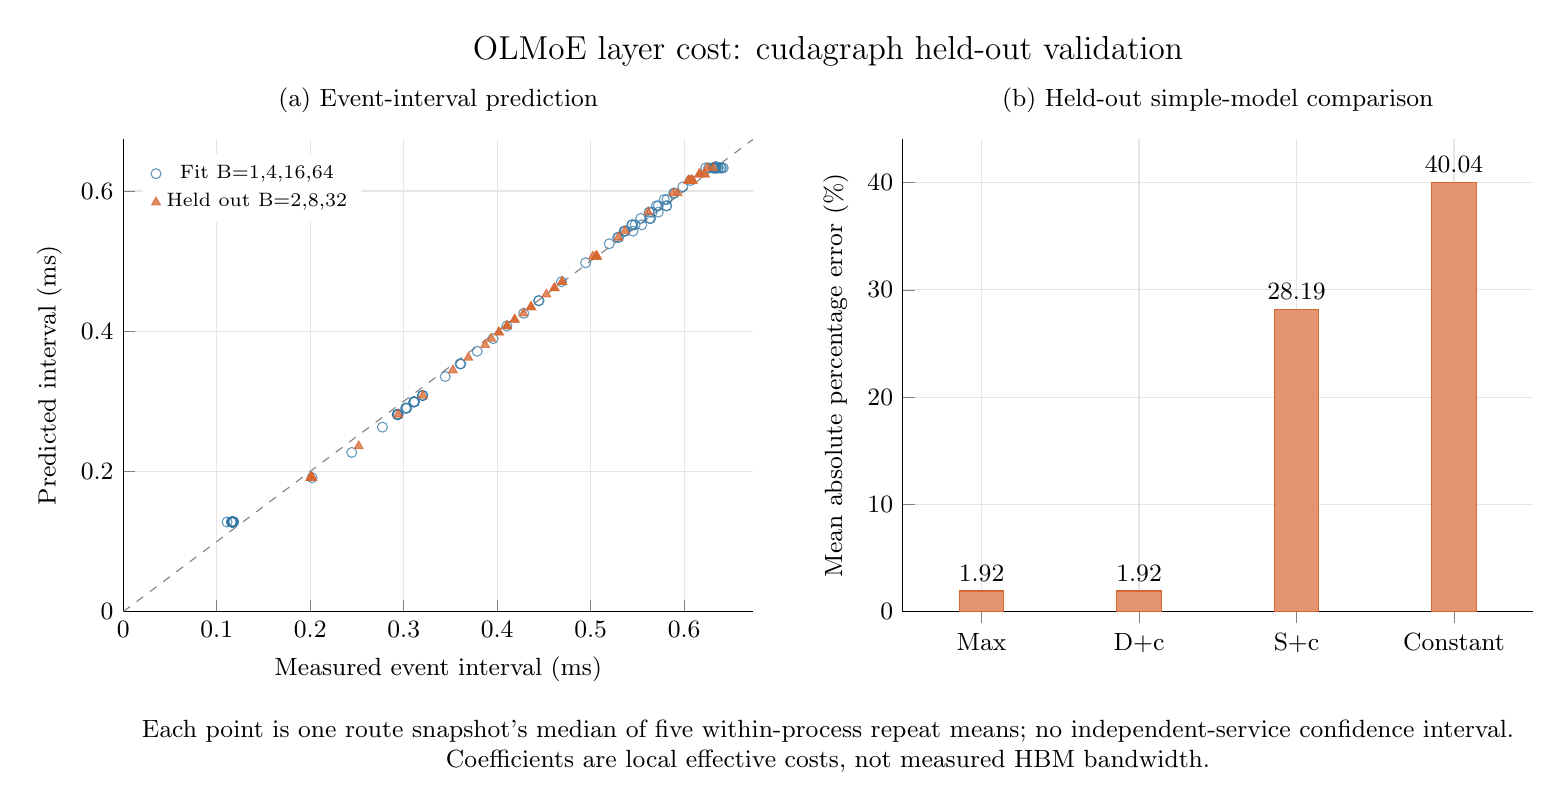
\begin{tikzpicture}
\definecolor{cal}{HTML}{3478A5}\definecolor{test}{HTML}{D76832}\definecolor{profile}{HTML}{3B8A5A}
\begin{groupplot}[group style={group size=2 by 1,horizontal sep=1.9cm},width=8.0cm,height=6.0cm,scale only axis,axis lines*=left,grid=major,grid style={gray!20},tick label style={font=\small},label style={font=\small},title style={font=\small},legend style={font=\scriptsize,draw=none},unbounded coords=jump]
\nextgroupplot[title={(a) Event-interval prediction},xlabel={Measured event interval (ms)},ylabel={Predicted interval (ms)},xmin=0,xmax=0.6739118434488773,ymin=0,ymax=0.6739118434488773,legend pos=north west]\addplot[only marks,color=cal,mark=o,mark size=1.8pt,opacity=0.75] coordinates {(0.110998399928,0.127908110094) (0.115934399515,0.127908110094) (0.117078400776,0.127908110094) (0.201950401068,0.191034303735) (0.117548799887,0.127908110094) (0.117609600723,0.127908110094) (0.244392001629,0.227106414387) (0.117896000296,0.127908110094) (0.117817600071,0.127908110094) (0.277267198265,0.263178525039) (0.116880000383,0.127908110094) (0.115915200859,0.127908110094) (0.320136001706,0.308268663353) (0.116900800169,0.127908110094) (0.115707199648,0.127908110094) (0.344438400865,0.335322746342) (0.116561599448,0.127908110094) (0.11618719995,0.127908110094) (0.361145597696,0.353358801668) (0.1165551994,0.127908110094) (0.116174399108,0.127908110094) (0.378593598306,0.371394856994) (0.293969604373,0.281214580365) (0.293772797287,0.281214580365) (0.311689600348,0.299250635691) (0.360225600004,0.353358801668) (0.302180796862,0.290232608028) (0.319969598949,0.308268663353) (0.395662401617,0.38943091232) (0.303403197229,0.290232608028) (0.320459201932,0.308268663353) (0.444790403545,0.443539078298) (0.293235197663,0.281214580365) (0.311136001348,0.299250635691) (0.468742400408,0.470593161287) (0.29308000356,0.281214580365) (0.30223840028,0.290232608028) (0.410270397365,0.407466967646) (0.293595196307,0.281214580365) (0.310769598186,0.299250635691) (0.428377598524,0.425503022972) (0.293566399813,0.281214580365) (0.310913601518,0.299250635691) (0.444166401029,0.443539078298) (0.529942396283,0.533719354928) (0.543870401382,0.551755410253) (0.544593596458,0.551755410253) (0.578705608845,0.587827520905) (0.536467194557,0.54273738259) (0.547494399548,0.551755410253) (0.562496000528,0.569791465579) (0.528804802895,0.533719354928) (0.553551998734,0.560773437916) (0.589316800237,0.596845548568) (0.519867199659,0.524701327265) (0.565790396929,0.569791465579) (0.588951998949,0.596845548568) (0.494542402029,0.497647244276) (0.570278391242,0.578809493242) (0.598518392444,0.605863576231) (0.535856002569,0.54273738259) (0.572347199917,0.578809493242) (0.606729596853,0.614881603894) (0.536868798733,0.54273738259) (0.581707200408,0.587827520905) (0.623159998655,0.63291765922) (0.626230403781,0.63291765922) (0.545276802778,0.54273738259) (0.630609604716,0.63291765922) (0.631995198131,0.63291765922) (0.554686403275,0.551755410253) (0.631600001454,0.63291765922) (0.636255997419,0.63291765922) (0.564127999544,0.560773437916) (0.632934400439,0.63291765922) (0.638841602206,0.63291765922) (0.563015991449,0.560773437916) (0.63351200819,0.63291765922) (0.632219204307,0.63291765922) (0.572356802225,0.569791465579) (0.636552006006,0.63291765922) (0.634099203348,0.63291765922) (0.581292805076,0.578809493242) (0.640147200227,0.63291765922) (0.634337595105,0.63291765922) (0.581081601977,0.578809493242) (0.641820803285,0.63291765922) (0.634059199691,0.635026505563)};
\addlegendentry{Fit B=1,4,16,64}
\addplot[only marks,color=test,mark=triangle*,mark size=1.8pt,opacity=0.75] coordinates {(0.202204799652,0.191034303735) (0.200697600842,0.191034303735) (0.20178880021,0.191034303735) (0.251833599061,0.23612444205) (0.200820799172,0.191034303735) (0.200766400993,0.191034303735) (0.2940576002,0.281214580365) (0.201596798748,0.191034303735) (0.201014402509,0.191034303735) (0.320472002029,0.308268663353) (0.201831998676,0.191034303735) (0.201035200059,0.191034303735) (0.352627201378,0.344340774005) (0.200937599689,0.191034303735) (0.20032640025,0.191034303735) (0.36913279891,0.362376829331) (0.200568000227,0.191034303735) (0.200289601088,0.191034303735) (0.387145602703,0.380412884657) (0.200952000171,0.191034303735) (0.200787201524,0.191034303735) (0.418542401493,0.416484995309) (0.410593600571,0.407466967646) (0.428153601289,0.425503022972) (0.436108799279,0.434521050635) (0.460971200466,0.461575133624) (0.418863999844,0.416484995309) (0.436060801148,0.434521050635) (0.502361604571,0.506665271939) (0.401726400852,0.398448939983) (0.43640639782,0.434521050635) (0.529643201828,0.533719354928) (0.401951999962,0.398448939983) (0.452656002343,0.452557105961) (0.536676800251,0.54273738259) (0.410608001053,0.407466967646) (0.461543999612,0.461575133624) (0.56155680418,0.569791465579) (0.410251201689,0.407466967646) (0.469438400865,0.470593161287) (0.588377600908,0.596845548568) (0.393700799346,0.38943091232) (0.46961439997,0.470593161287) (0.604449597001,0.614881603894) (0.604631996155,0.614881603894) (0.506279993057,0.506665271939) (0.593030399084,0.596845548568) (0.604742395878,0.614881603894) (0.50573759973,0.506665271939) (0.607057598233,0.614881603894) (0.607486397028,0.614881603894) (0.505619198084,0.506665271939) (0.608865594864,0.614881603894) (0.608592003584,0.614881603894) (0.505913609266,0.506665271939) (0.609145602584,0.614881603894) (0.616056004167,0.623899631557) (0.506609603763,0.506665271939) (0.616199997067,0.623899631557) (0.621681603789,0.623899631557) (0.50637280345,0.506665271939) (0.617164802551,0.623899631557) (0.631112000346,0.63291765922) (0.506728002429,0.506665271939) (0.622313600779,0.623899631557) (0.624988797307,0.63291765922)};
\addlegendentry{Held out B=2,8,32}\addplot[gray,dashed,forget plot,domain=0:0.6739118434488773] {x};
\nextgroupplot[title={(b) Held-out simple-model comparison},ylabel={Mean absolute percentage error (\%)},ybar,bar width=16pt,xtick={1,2,3,4},xticklabels={Max,D+c,S+c,Constant},ymin=0,xmin=0.5,xmax=4.5,nodes near coords,point meta=y,every node near coord/.append style={font=\small,/pgf/number format/fixed,/pgf/number format/precision=2}]\addplot[fill=test!70,draw=test] coordinates {(1,1.9204815257) (2,1.92401933778) (3,28.1860170997) (4,40.0408721708)};
\end{groupplot}
\path (group c1r1.north west) -- node[above=0.8cm,font=\large] {OLMoE layer cost: cudagraph held-out validation} (group c2r1.north east);
\path (group c1r1.south west) -- node[below=1.25cm,align=center,font=\small] {Each point is one route snapshot's median of five within-process repeat means; no independent-service confidence interval.\\Coefficients are local effective costs, not measured HBM bandwidth.} (group c2r1.south east);
\end{tikzpicture}\end{document}
